\documentclass{standalone}
\usepackage{tikz}

\usepackage{color}

\usetikzlibrary{arrows.meta}
\usetikzlibrary{calc}
\usetikzlibrary{shapes}
\usetikzlibrary{bending}
\usetikzlibrary{patterns}

\usepackage{gensymb}

\usepackage{pgfplots}
\usepgfplotslibrary{polar}

\begin{document}
		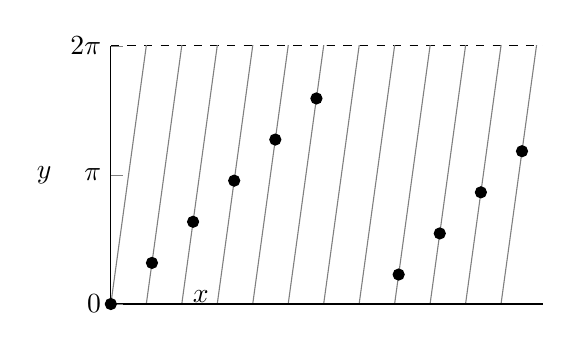
\begin{tikzpicture}[
	% scale=0.8,
	]	
	

	\begin{axis}[
	scale=0.8,
	axis on top=true,
	unit vector ratio=1 1,
	axis x line*=middle, axis y line*=middle,
	xtick=\empty,
	ytick=\empty,
	extra y ticks= {0, 3.14, 6.28},
	extra y tick labels = {0, $\pi$, $2\pi$},
	xlabel=$x$,
	ylabel=$y$,
	ylabel style={rotate=-90},
	x label style={right=-16mm, above=-1mm},
	ymin=0, ymax=6.28, 
	xmin=0, xmax=10.5, 
	]
	
	\addplot[dashed,domain=0:10.5] {6.28};
		
	\addplot[mark=*,domain=0:10, only marks, samples=11] {mod(x,2*pi)};
	
	\addplot[color=gray, domain=0:10]  {(2*pi+1)*x};
	\addplot[color=gray, domain=0:10]  {(2*pi+1)*x-2*pi};
	\addplot[color=gray, domain=0:10]  {(2*pi+1)*x-2*2*pi};
	\addplot[color=gray, domain=0:10]  {(2*pi+1)*x-3*2*pi};	
	\addplot[color=gray, domain=0:10]  {(2*pi+1)*x-4*2*pi};
	\addplot[color=gray, domain=0:10]  {(2*pi+1)*x-5*2*pi};
	\addplot[color=gray, domain=0:10]  {(2*pi+1)*x-6*2*pi};
	\addplot[color=gray, domain=0:10]  {(2*pi+1)*x-7*2*pi};
	\addplot[color=gray, domain=0:10]  {(2*pi+1)*x-8*2*pi};		
	\addplot[color=gray, domain=0:10]  {(2*pi+1)*x-9*2*pi};
	\addplot[color=gray, domain=0:10]  {(2*pi+1)*x-10*2*pi};
	\addplot[color=gray, domain=0:10.5]  {(2*pi+1)*x-11*2*pi};
	
	\end{axis}
	
	
	\end{tikzpicture}  
\end{document}